%        File: task-oriented_parser_evaluation.tex
%     Created: 周五 三月 02 04:00 下午 2012 W EST
% Last Change: 周五 三月 02 04:00 下午 2012 W EST
%
\documentclass[a4paper]{article}
\usepackage{hyperref}
\usepackage{graphicx}
%\usepackage{gb4e}
%\usepackage{longtable}
\usepackage[style=authoryear,natbib=true]{biblatex}
\bibliography{D:/Research/bib/Parsing}
%\usepackage{graphicx}
\usepackage{algorithm}
\usepackage{algorithmic}
\usepackage{lingmacros}
\usepackage{tikz}
\usepackage{tikz-qtree}
%\usepackage{gb4e}
\title{Lexicalized Tree Adjoining Grammar Extraction For KBGEN}
\author{Wei Qiu \and Jiri Marsik}
%\date{}
\begin{document}
\maketitle
\begin{abstract}
\end{abstract}
\section{Introduction}
\section{Semantic Annotation}
\label{sec:sem-annot}
\subsection{Annotation guidelines}
\subsection{Problems}


\section{Preprocessing}

\subsection{Parsing with head information}

Our plan is to extract the elementary trees for a TAG from a treebank.
Since our corpus lacks phrase structure information, we ran an
off-the-shelf parser on it. The parser that we used for this task is
the Stanford parser.

At the outset, we had plans to use both the phrase structure and
dependency parses that the Stanford parser could produce. Previous
research has shown that having a dependency parse facilitates the task
of determining headedness, which is usually a subtask of elementary
tree extraction.

Finally, we have found a simpler way of getting the head information
directly in the phrase structure parse trees through a command line
switch in the Stanford parser.


Furthermore, the Stanford parser offers two pre-trained models for
parsing English, an unlexicalized one and a lexicalized one. We have
done the parsing using both of them and try to review their
performance. Their outputs were significantly different and both
performed their own idiosyncratic errors. We judged which of these
errors would likely be more harmful to the following grammar
extraction process and decided to stick with the output of the
unlexicalized parser (though the result of the unlexicalized parsing
almost as just as bad as that of the lexicalized one).

\subsection{Conjunction resolving}

When we started working on the manual alignment with our self-enforced
constraint to produce only contiguous groups (see section
\ref{sec:sem-annot}), one of the difficulties we faced was
coordination. Consider the following example:

\begin{verbatim}
Electrogenic pumps, which consist of a hydrophobic amino acid,
a polar amino acid and a monomer, create  membrane potential.

(KBGEN-INPUT 
    :TRIPLES (
            (|Electrogenic-Pump21300| |has-part| |Monomer21323|)
            (|Electrogenic-Pump21300| |has-part| |Polar-Amino-Acid21291|)
            (|Electrogenic-Pump21300| |has-part| |Hydrophobic-Amino-Acid21290|)
            (|Create21297| |agent| |Electrogenic-Pump21300|)
            (|Create21297| |result| |Membrane-Potential21299|))
    :INSTANCE-TYPES (
            (|Monomer21323| |instance-of| |Monomer|)
            (|Polar-Amino-Acid21291| |instance-of| |Polar-Amino-Acid|)
            (|Hydrophobic-Amino-Acid21290| |instance-of| |Hydrophobic-Amino-Acid|)
            (|Electrogenic-Pump21300| |instance-of| |Electrogenic-Pump|)
            (|Create21297| |instance-of| |Create|)
            (|Membrane-Potential21299| |instance-of| |Membrane-Potential|)))
\end{verbatim}

How should the group that contains the word \emph{consists} look like?
It takes an indirect object starting with \emph{of}, so we make
\emph{of} part of the same group. Since this verb is the head of a
relative clause that modifies an NP, we would like to have the first
comma and the word \emph{which} in the same group as well. So far so
good, we have a contiguous group, ``\emph{, which consists of}''. The
set of triples that corresponds to this group is the set of the three
triples with the \textbf{has-part} relation.

So far so good (omitting the final comma, that is). But now we have
trouble when we look at the object of \emph{consists}. To what group
should the comma and the conjunction \emph{and} belong, i.e. what
semantics correspond to them and only to them?

To resolve this issue, we have developed a tool to reify the
coordination structures within the triples themselves.

In our first approach, our program would look for every instance where
one entity was in the same relation with multiple entities, such as
above, and converted the triples to the following:

\begin{verbatim}
:TRIPLES (
        (|Coordination2085| |coordinates| |Monomer21323|)
        (|Coordination2085| |coordinates| |Polar-Amino-Acid21291|)
        (|Coordination2086| |coordinates| |Coordination2085|)
        (|Coordination2086| |coordinates| |Hydrophobic-Amino-Acid21290|)
        (|Electrogenic-Pump21300| |has-part| |Coordination2086|)
        (|Create21297| |agent| |Electrogenic-Pump21300|)
        (|Create21297| |result| |Membrane-Potential21299|))
\end{verbatim}

In this approach, we build a very specific kind of binary tree which
covers the coordinated entities (the generated tree is specific in
that it always leans to the right, so it looks more like a linked
list). Here, one \textbf{Coordination} entity,
\textbf{Coordination2085}, subsumes the \textbf{Monomer21323} and the
\textbf{Polar-Amino-Acid21291}. This coordination corresponds to the
conjunction \emph{and}. The second coordination connects another
entity, the \textbf{Hydrophobic-Amino-Acid21290}, to the previously
formed \textbf{Coordination2085}. The resulting
\textbf{Coordination2086} can then serve as the singular object to the
verb \emph{consists}. Now, all of the NP coordinating constructs
(commas and \emph{and}) are easily accounted for. They form singleton
groups that are aligned to a pair of \textbf{coordinates} relations.

Once we made the switch from contiguous groups, we revised our
approach to coordination. Instead of making this hierarchy of
coordination constructs, we just create a single \textbf{Coordination}
entity which encapsulates all of the coordinated entities directly.
Obviously, this would not have been possible for coordinations of more
than 2 constituents using only contiguous groups, since we would not
to place two non-adjacent conjunction markers into one group.

The upsides of this new approach are that it reduces the complexity of
the newly added triples and that it does not overgenerate like the
last approach, which would end up extracting two elementary trees for
conjunction (one for comma and one for \emph{and}), but would not be
able to distinguish between them and use them properly. The only
downside of the new approach is that it needs to learn different
elementary trees for each different arity of conjunction present in
the corpus. However, since the number of coordinated constituents is
always between 2 and 4 in our corpus, this is a non-issue.

Here is the above example, now rendered using the new coordination
aggregation rules:

\begin{verbatim}
    :TRIPLES (
            (|Electrogenic-Pump21300| |has-part| |Coordination2015|)
            (|Coordination2015| |coordinates| |Monomer21323|)
            (|Coordination2015| |coordinates| |Polar-Amino-Acid21291|)
            (|Coordination2015| |coordinates| |Hydrophobic-Amino-Acid21290|)
            (|Create21297| |agent| |Electrogenic-Pump21300|)
            (|Create21297| |result| |Membrane-Potential21299|))
\end{verbatim}

The code for performing the former aggregation method is still present
in the aggregation program, but is no longer used (see function
\texttt{coordinate-objects-list}). Switching to the new method was
just a matter of writing a new function,
\texttt{coordinate-objects-flat}, and calling that one instead of the
former.

\subsection{Normalizing}

\section{TAG extraction}
After we get the normalized tree with head information, we can extract the TAG from it with the help of the alignment of surface sentence to underlying KBGEN triples.
The key idea is extract adjunction trees greedily, then extract the substitution trees. Of course conjunction trees as a specific form of substitution trees require
some special treatment before adjunction trees can be extracted.

First we will present the pseudo code Algorithm \ref{alg:tag_extract}, \ref{alg:extract_conj}, \ref{alg:extract_adj}, \ref{alg:extract_sub} for the tree extraction algorithms, then a working example will be given to illustrate the idea.
\begin{algorithm}
    \caption{LTAG extraction algorithm}
    \label{alg:tag_extract}
    \begin{algorithmic}[1]
        \REQUIRE $Tree$, $alignment$ 
        \FORALL{$node$ in $Tree$}
        \STATE add semantic group information according to $alignment$
        \ENDFOR
        \STATE $agenda \Leftarrow [Tree]$
        \STATE $well\_formed\_tree \Leftarrow []$
        \WHILE {$agenda$ is not empty}
            \STATE $current\_tree = agenda.pop() $
            \IF{$current\_tree$ only contains one group}
            \STATE $well\_formed\_tree.append(.current\_tree)$
            \ENDIF
            \STATE extract conjunction subpart
            \STATE extract adjunction subpart
            \IF {adjunction found}
                \STATE continue
            \ELSE
                \STATE extract substitution subpart
            \ENDIF
        \ENDWHILE
        \RETURN $well\_formed\_tree$
    \end{algorithmic}
\end{algorithm}

\begin{algorithm}
    \caption{extract conjunction subpart}
    \label{alg:extract_conj}
    \begin{algorithmic}[1]
        \FORALL {$subtree$ in $Tree$}
            \IF{$subtree$ has a conjunction structure}
                \STATE cut the conjunction tree off the subtree
                \STATE remove all arguments in the conjunction structure
                \STATE copy group information as candidate information
                %\COMMENT{This information is for semantic alignment afterwards}
                \STATE change the empty node'group to empty set
                \STATE update the group information of all separated parts 
                \STATE put subtree, conjunction tree, argument trees into $agenda$
            \ENDIF
        \ENDFOR
    \end{algorithmic}
\end{algorithm}

\begin{algorithm}
    \caption{extract adjunction subpart}
    \label{alg:extract_adj}
    \begin{algorithmic}[1]
        \FORALL {$subtree$ in $Tree$}
            \FORALL {leftmost child or rightmost child of $subtree$}
                \STATE TODO
                \IF {$child$ has the same pos as $subtree$}
                    \IF {$child$ is well separated from other parts}
                        \STATE cut off $subtree$ from its parent
                        \STATE copy the group information as candidate information
                        \STATE update the hole's group as empty set
                        \STATE cut off $child$ from $subtree$
                        \STATE copy the group information of $child$ hole as candidate information
                        \STATE update $child$ hole's group as empty set
                        \STATE update group information of all subparts
                        \STATE put adjunction mark
                        \STATE put all subparts into $agenda$
                    \ENDIF
                \ENDIF
            \ENDFOR
        \ENDFOR
    \end{algorithmic}
\end{algorithm}

\begin{algorithm}
    \caption{extract substituition subpart}
    \label{alg:extract_sub}
    \begin{algorithmic}[1]
        \STATE $headgroup \Leftarrow current\_tree's head group$
        \FORALL {$subtree$ in $current\_tree$}
        \IF{$subtree$'s group is disjoint from $headgroup$}
            \STATE cut $subtree$ off $current_tree$
            \STATE copy the relative group information to candidate
            \STATE update all group information
            \STATE put substitution mark
        \ENDIF
        \ENDFOR
    \end{algorithmic}
\end{algorithm}

We will take sentence

\enumsentence{The rate of detoxification in the liver cell is directly proportional to the quantity of smooth endoplasmic reticulum in the liver cell.}

as example, the semantic group annotation is:

\enumsentence{[1 The rate of] [2 detoxification] [3 in] [4 the liver cell] [5 is directly proportional to] [6 the quantity of] [7 smooth endoplasmic reticulum] [8 in] [9 the liver cell] .}
After parsing and preprocessing, we get the tree:

\begin{center}
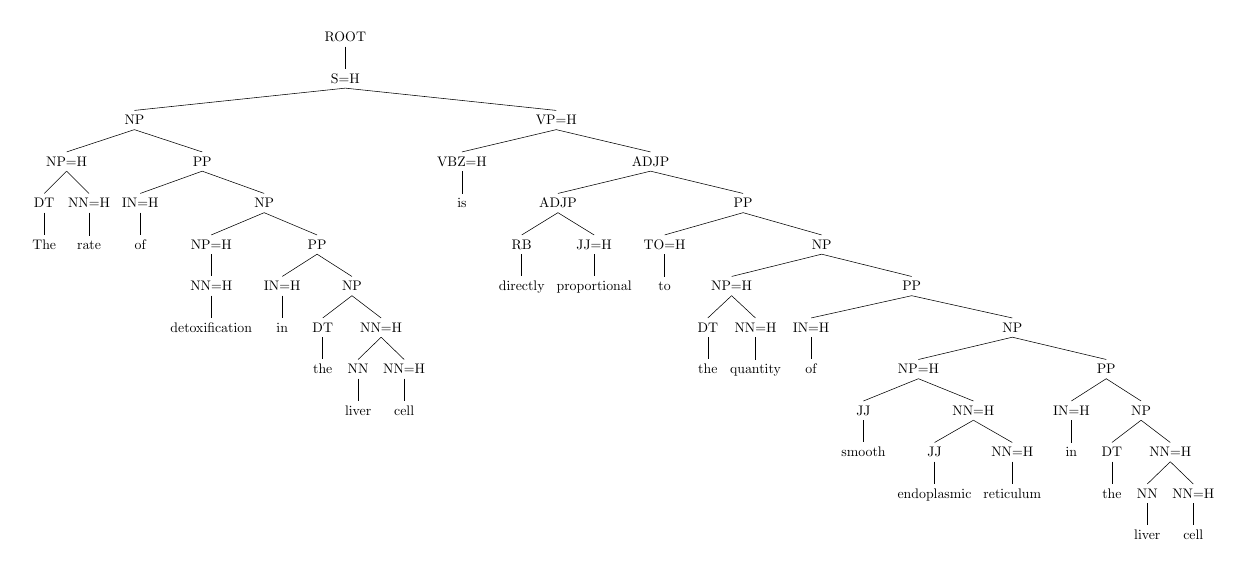
\begin{tikzpicture}[scale=0.5]
\Tree [.ROOT [.S=H [.NP [.NP=H [.DT The ] [.NN=H rate ] ] [.PP [.IN=H of ] [.NP [.NP=H [.NN=H detoxification ] ] [.PP [.IN=H in ] [.NP [.DT the ] [.NN=H [.NN liver ] [.NN=H cell ] ] ] ] ] ] ] [.VP=H [.VBZ=H is ] [.ADJP [.ADJP [.RB directly ] [.JJ=H proportional ] ] [.PP [.TO=H to ] [.NP [.NP=H [.DT the ] [.NN=H quantity ] ] [.PP [.IN=H of ] [.NP [.NP=H [.JJ smooth ] [.NN=H [.JJ endoplasmic ] [.NN=H reticulum ] ] ] [.PP [.IN=H in ] [.NP [.DT the ] [.NN=H [.NN liver ] [.NN=H cell ] ] ] ] ] ] ] ] ] ] ] ]
\end{tikzpicture}
\end{center}

$S=H$ label means the syntax category is S and S is the head of its parent tree. We can see that stanford parser doesn't always provide head information. For example:
\begin{center}
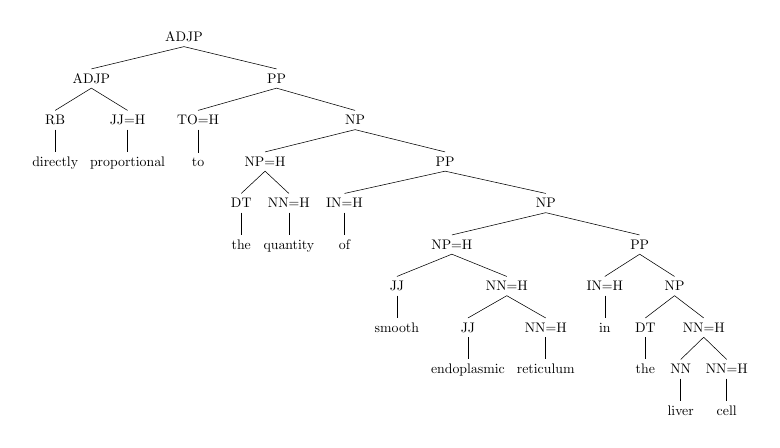
\begin{tikzpicture}[scale=0.5]
\Tree [.ADJP [.ADJP [.RB directly ] [.JJ=H proportional ] ] [.PP [.TO=H to ] [.NP [.NP=H [.DT the ] [.NN=H quantity ] ] [.PP [.IN=H of ] [.NP [.NP=H [.JJ smooth ] [.NN=H [.JJ endoplasmic ] [.NN=H reticulum ] ] ] [.PP [.IN=H in ] [.NP [.DT the ] [.NN=H [.NN liver ] [.NN=H cell ] ] ] ] ] ] ] ] ]
\end{tikzpicture}
\end{center}
All of the children of root ADJP don't have any head information. This is a problem for our extraction algorithm simply because our algorithm relies on the head information to find the real group for the root. And quite often the head itself would be extracted out leaving a hole in the original tree. We need also to assign a head to the remaining siblings of it. Our work around is to assign the first child which has non-empty group informaiton as the head. This may seem to be problematic, but actually it works pretty well simply because the tree is almost binarized And stanford parser generate head information for the most cases. Of course, a heuristic rule may work better. We here leave it to future work. Check $extractor.\_get\_head\_group$ for the details.

First the whole tree will be added to agenda. After it has been poped out for further examination, firstly it will be checked whether it contains any conjunctions. The answer is no in this case. Then we can check whether it contains any adjuctions.

A simple strategy is to only check the root and its leftmost and rightmost children. But a close look into the corpus show us this strategy is too simple and sometimes will not work. It will extrat some grammars without good linguistic interpretation if we postpone the adjuction checking of other subtrees. So in our algorithm, we exaustively check the adjunction for all of the subtrees. An example that the simple strategy doesn't work is shown below:

\begin{center}
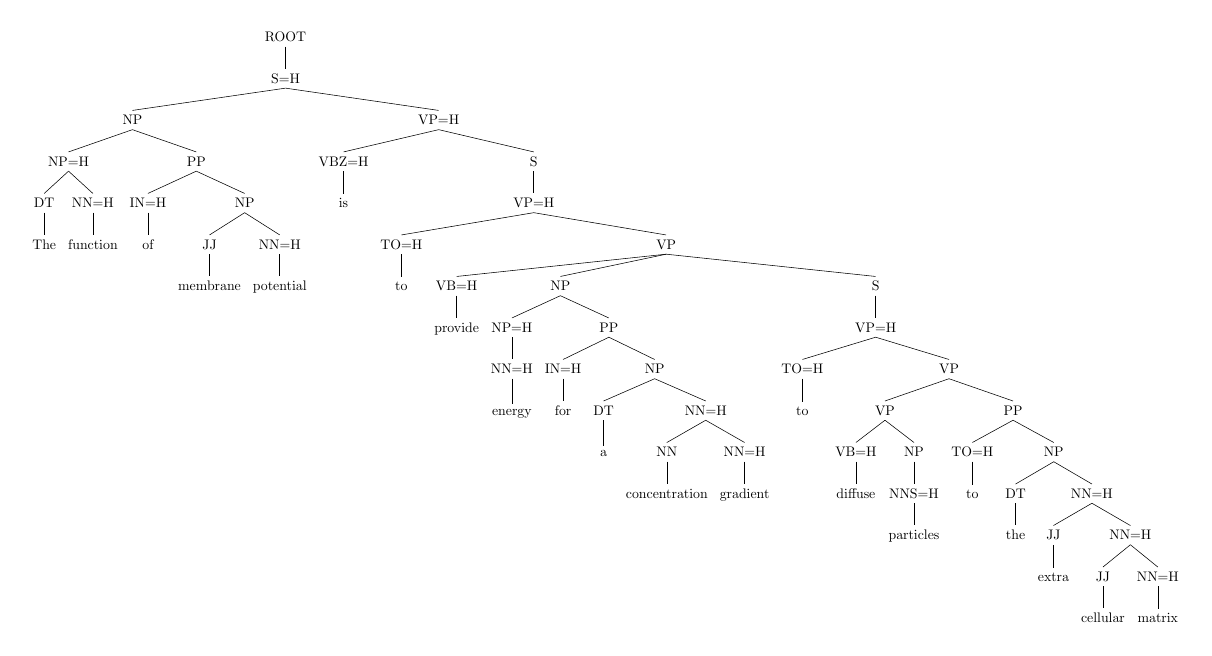
\begin{tikzpicture}[scale=0.5]
\Tree [.ROOT [.S=H [.NP [.NP=H [.DT The ] [.NN=H function ] ] [.PP [.IN=H of ] [.NP [.JJ membrane ] [.NN=H potential ] ] ] ] [.VP=H [.VBZ=H is ] [.S [.VP=H [.TO=H to ] [.VP [.VB=H provide ] [.NP [.NP=H [.NN=H energy ] ] [.PP [.IN=H for ] [.NP [.DT a ] [.NN=H [.NN concentration ] [.NN=H gradient ] ] ] ] ] [.S [.VP=H [.TO=H to ] [.VP [.VP [.VB=H diffuse ] [.NP [.NNS=H particles ] ] ] [.PP [.TO=H to ] [.NP [.DT the ] [.NN=H [.JJ extra ] [.NN=H [.JJ cellular ] [.NN=H matrix ] ] ] ] ] ] ] ] ] ] ] ] ] ]
\end{tikzpicture}
\end{center}
When 
\begin{center}
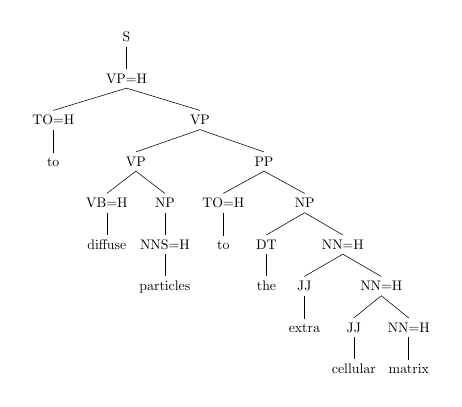
\begin{tikzpicture}[scale=0.5]
\Tree [.S [.VP=H [.TO=H to ] [.VP [.VP [.VB=H diffuse ] [.NP [.NNS=H particles ] ] ] [.PP [.TO=H to ] [.NP [.DT the ] [.NN=H [.JJ extra ] [.NN=H [.JJ cellular ] [.NN=H matrix ] ] ] ] ] ] ] ]
\end{tikzpicture}
\end{center}
is popped out, if we don't identify the adjuction structure wrapped inside, the substitution procedure would break it and it would be impossible to find a proper adjuction tree.

Now come back to our example, the chuck ``The rate of detoxification in the liver cell'' looks like a adjuction structure for its first left child, but actually it's not simply because the adjunction node's group is not disjoint from other parts(``of'' is also in group 1). It's illustrated in Figure \ref{fig:no-adjunct}.

\begin{figure}[h]
    \begin{center}
        \includegraphics[scale=0.4]{noadj.ps}
    \end{center}
    \caption{``The rate'' is not adjuction}
    \label{fig:no-adjunct}
\end{figure}

Using the same algorithm, we can identify ``the rate of '' is a proper adjuction tree.

The third step is to extract the emlemtary tree. Actually after all of conjuctions and adjuctions are kicked out the leftover's root must be a root of elementary tree. Based on this observation, the algorithm for substitution tree extraction is relatively simple. First we identify the group of the root, then kick out all the parts which don't belong to this group and add them to the agenda. The left spine would be a ``pure'' elementary tree which can be directly add to the resulted grammar.

For this example, 9 grammar snippets will be extracted:

\begin{figure}[h]
    \begin{center}
        \includegraphics[scale=0.5]{1.eps}
    \end{center}
    \caption{1}
\end{figure}
\begin{figure}[h]
    \begin{center}
        \includegraphics[scale=0.5]{2.eps}
    \end{center}
    \caption{2}
\end{figure}
\begin{figure}[h]
    \begin{center}
        \includegraphics[scale=0.5]{3.eps}
    \end{center}
    \caption{3}
\end{figure}
\begin{figure}[h]
    \begin{center}
        \includegraphics[scale=0.5]{4.eps}
    \end{center}
    \caption{4}
\end{figure}
\begin{figure}[h]
    \begin{center}
        \includegraphics[scale=0.5]{5.eps}
    \end{center}
    \caption{5}
\end{figure}
\begin{figure}[h]
    \begin{center}
        \includegraphics[scale=0.5]{6.eps}
    \end{center}
    \caption{6}
\end{figure}
\begin{figure}[h]
    \begin{center}
        \includegraphics[scale=0.5]{7.eps}
    \end{center}
    \caption{7}
\end{figure}
\begin{figure}[h]
    \begin{center}
        \includegraphics[scale=0.5]{8.eps}
    \end{center}
    \caption{8}
\end{figure}
\begin{figure}[h]
    \begin{center}
        \includegraphics[scale=0.5]{9.eps}
    \end{center}
    \caption{9}
\end{figure}
\section{Semantic roles alignment}
The extraction step extract grammar snippets for each sentence. This step intends to align the semantics to the grammar snippets and the syntax holes in the grammar snippets.


\section{Implementation and result}
data format
\section{Conclusion \& Future work}
\subsection{Future work}
\begin{itemize}
    \item workaround with parsing errors.
    \item more robust extraction algorithms
    \item more robust alignment algorithms
\end{itemize}
\end{document}
